%\begin{evenBlock}{Gate Dribbling (10 min)}
%Set up 3 gates in a zig-zag pattern about 6 to 10 yards apart.  The gates should be about a yard wide or less depending on dribbling skill of the group.  Players start a the end line and dribble through the gates as fast as possible.  Use the same technique as the previous drill.
%\end{evenBlock}

\begin{oddBlock}{Cross-Hairs}

\begin{minipage}[t]{\linewidth}
    \centering
    
    \begin{minipage}{.3\linewidth} % Left column and width
        
        \centering
        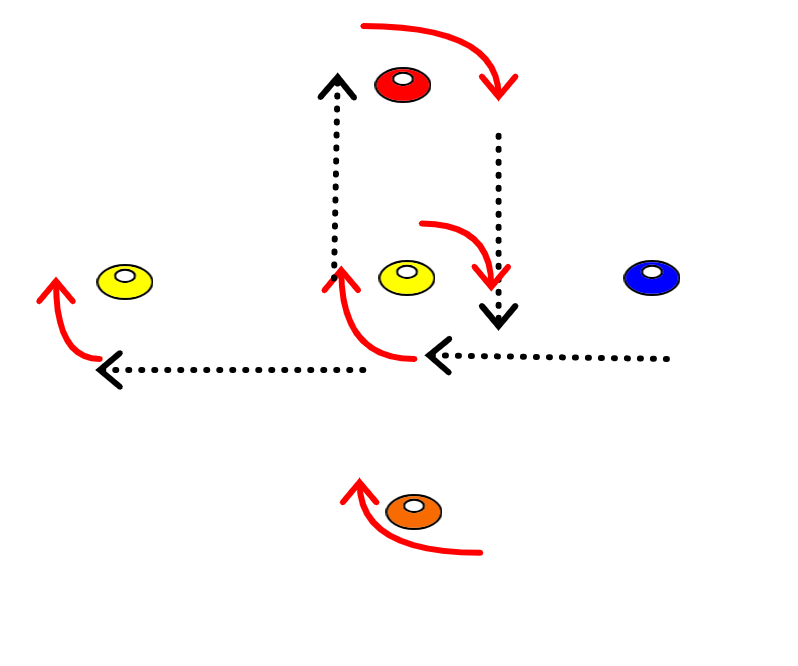
\includegraphics[width=.6\textwidth]{../img/Trimmed/cross_hairs}

    \end{minipage}
    \hspace{0.05\linewidth}
    \begin{minipage}{.6\linewidth} % Left column and width
        \textbf{Drill Description:}
        
        \begin{enumerate}
        \setlength{\itemsep}{0pt}
        \setlength{\parskip}{0pt}
        \setlength{\parsep}{0pt}
        \item Players start at blue cone and race to the center cone turn right and race around the outer cones and always returning to the center cone.
        \item Finish by accelerating past the blue cone.
        \end{enumerate}
    \end{minipage}
\end{minipage}
%\vspace{12pt}
%
%    \textbf{Coaching Points:}
%    \begin{itemize}
%        \setlength{\itemsep}{0pt}
%        \setlength{\parskip}{0pt}
%        \setlength{\parsep}{0pt}
%        \item
%    \end{itemize}

\end{oddBlock}